\begin{pastexam}[label={px:nccu-115-dsa-12}]{政大資科所 115 學年度 第 12 題}
（問答）

The following code defines the structure of a binary search tree. Please answer the questions below.
\begin{minted}[fontsize=\small,escapeinside=||]{cpp}
#include <iostream>
#include <vector>
using namespace std;

struct TreeNode {
    int data;
    TreeNode* left;
    TreeNode* right;
    TreeNode(int val) : data(val), left(nullptr), right(nullptr) {}
};
TreeNode* insertNode(TreeNode* root, int data) {
    if (root == nullptr) {
        return new TreeNode(data);
        }
    if (data < root->data) {
        root->left = |\underline{\textbf{blank1}}|;}
    else if (data > root->data) {
        root->right = |\underline{\textbf{blank2}}|;}
    return root;
}

void Traversal(TreeNode* root) {
    if (root != nullptr) {
        Traversal(root->left);
        cout << root->data << " ";
        Traversal(root->right);
    }
}

int main() {
    TreeNode* root = nullptr;
    vector<int> initial_data = {20, 30, 70, 15, 40, 55, 80};
    for (int val : initial_data) {
        root = insertNode(root, val);
    }

    cout << "Order 1: ";
    Traversal(root);
    cout << endl;
    int new_value = 45;
    root = insertNode(root, new_value);
    cout << "Order 2: ";
    Traversal(root);
    cout << endl;
    return 0;
}
\end{minted}
(a) (5\%) What should be filled in \textbf{blank1} and \textbf{blank2}?\\
(b) (5\%) What is the output of the code?\\
(c) (5\%) Which traversal order of the output is used?\\
(d) (5\%) Based on the final binary search tree (after the insertion of 45), what is the output sequence for
the post-order traversal?
\end{pastexam}

\begin{pastsoln}
本題屬資結書第~9~章（插入）和第~7.3~節（走訪）。

\textbf{(a)} 遞迴插入（資結書第~9.2~節）：新鍵比根小就插進左子樹，比根大就插進右子樹，並把遞迴回傳的
子樹根接回去（子樹原本是空的時候，回傳的是新節點，要接上父節點的指標）。
\begin{itemize}
\item blank1：\texttt{insertNode(root->left, data)}
\item blank2：\texttt{insertNode(root->right, data)}
\end{itemize}
和 \texttt{data} 相等的鍵兩個分支都不進，直接回傳 \texttt{root}，所以重複的鍵不會插入。

\textbf{(b)} 依序插入 $20, 30, 70, 15, 40, 55, 80$：
\begin{itemize}
\item $20$ 是根；$30 > 20$，當 $20$ 的右兒子；$70 > 20$、$> 30$，當 $30$ 的右兒子；$15 < 20$，當 $20$ 的
左兒子。
\item $40$：$> 20$、$> 30$、$< 70$，當 $70$ 的左兒子。 $55$：$> 20$、$> 30$、$< 70$、$> 40$，當 $40$ 的
右兒子。 $80$：$> 20$、$> 30$、$> 70$，當 $70$ 的右兒子。
\item 之後插入 $45$：$> 20$、$> 30$、$< 70$、$> 40$、$< 55$，當 $55$ 的左兒子。
\end{itemize}
最後的樹（虛線是後來插入的 $45$）：
\begin{center}
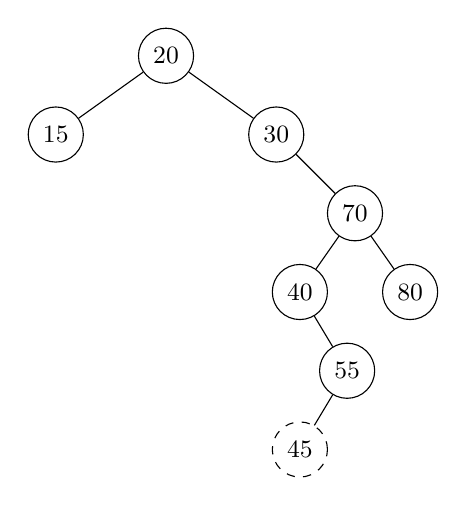
\begin{tikzpicture}[level distance=10mm,
  level 1/.style={sibling distance=28mm}, level 2/.style={sibling distance=20mm},
  level 3/.style={sibling distance=14mm}, level 4/.style={sibling distance=12mm},
  every node/.style={circle,draw,minimum size=7mm,inner sep=0pt,font=\small}]
\node {20}
  child {node {15}}
  child {node {30}
    child[missing] {}
    child {node {70}
      child {node {40}
        child[missing] {}
        child {node {55}
          child {node[dashed] {45}}
          child[missing] {}}}
      child {node {80}}}};
\end{tikzpicture}
\end{center}
\texttt{Traversal} 先走左子樹、再印根、再走右子樹，是中序走訪，二元搜尋樹的中序是由小到大
（資結書定理~9.1）。 每個數後面印一個空白，輸出是
\begin{minted}[fontsize=\small]{text}
Order 1: 15 20 30 40 55 70 80 
Order 2: 15 20 30 40 45 55 70 80 
\end{minted}
（兩行的行尾各有一個空白。）

\textbf{(c)} 中序走訪（in-order traversal，LVR）。

\textbf{(d)} 後序走訪是左子樹、右子樹、根（資結書第~7.3~節）。 從根 $20$ 開始展開：
\[
\text{post}(20) = \text{post}(15),\ \text{post}(30),\ 20,\quad
\text{post}(30) = \text{post}(70),\ 30,
\]
\[
\text{post}(70) = \text{post}(40),\ 80,\ 70,\quad
\text{post}(40) = \text{post}(55),\ 40,\quad
\text{post}(55) = 45,\ 55 .
\]
代回去得到
\[
15,\ 45,\ 55,\ 40,\ 80,\ 70,\ 30,\ 20 .
\]
\end{pastsoln}
